\documentclass{uebblatt}
\usepackage{stmaryrd}

\begin{document}

\maketitle{2}{\emph{Das ist das Koende, mein einziger Kofreund.}}
%\marginpar{\vspace*{-1cm}\hspace*{-0.5cm}\href{http://poesophicalbits.blogspot.de/2013/05/lambda-calculus-and-category-theory-in.html}{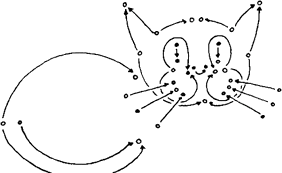
\includegraphics[angle=90,scale=0.5]{images/katzegorie}}}

% Kolimiten und Limiten vertauschen
% Limiten
% Enden
% Kan-Erweiterungen

\begin{aufgabe}{Beispiele für Limiten}
\begin{enumerate}
\item Zeige: In der Kategorie der~$k$-Vektorräume ist~$k[X]$ der Kolimes des
Diagramms $\bigl(k[X]_{\leq0} \lhra k[X]_{\leq1} \lhra k[X]_{\leq2} \lhra
\cdots \bigr)$. Dabei ist~$k[X]_{\leq n}$ der Unterraum der Polynome vom
Grad~$\leq n$. Was ist der Limes dieses Diagramms?
\item Finde ein Diagramm mit Limes~$k[[X]]$, dem Vektorraum
der formalen Potenzreihen!
\end{enumerate}
\end{aufgabe}

\begin{aufgabe}{Freie Konstruktionen}
\begin{enumerate}
\item Sei~$V : \mathrm{Vect}(k) \to \Set$ der Vergissfunktor und~$L : \Set \to
\mathrm{Vect}(k)$ der Funktor, der einer Menge~$X$ den freien~$k$-Vektorraum
auf~$X$ zuordnet. Beweise:~$L \dashv V$.
% Die Elemente von L(X) sind formale endliche Linearkombinationen sum_i a_i x_i
% mit Koeffizienten a_i aus k und x_i aus X.
\item Erkläre, was~"`$L \dashv V$"' anschaulich bedeutet!
Verwende \emph{Erzeuger} und \emph{Relationen}.
\item Finde Linksadjungierte zu den Vergissfunktoren~$\mathrm{Mon} \to \Set$
und~$\mathrm{Top} \to \Set$.
% Dabei ist~$\mathrm{Mon}$ die Kategorie der Monoide.
\end{enumerate}
\end{aufgabe}

\begin{aufgabe}{Das Tensorprodukt von Moduln als Koende}
Sei~$R$ ein Ring. Seien~$M$ ein Rechts-$R$-Modul
und~$N$ ein Links-$R$-Modul. Zeige:
\[ M \otimes_R N \cong \int^R M \otimes_\ZZ N. \]
% Dabei fassen wir~$R$ als Kategorie mit einem Objekt~$\star$ und
% Morphismen~$\Hom_R(\star,\star) = R$ auf; der Integrand ist der Funktor~$R^\op
% \times R \to \Ab$ mit~$(\star,\star) \mapsto M \otimes_\ZZ N$ und~$(r,r')
% \mapsto (x \otimes y \mapsto xr \otimes r'y)$.
\vspace{-1.5em}
\end{aufgabe}

\begin{aufgabe}{Die Limesformel für punktweise Kan-Erweiterungen}
Sei~$K : \M \to \C$ ein Funktor. Sei~$T : \M \to \A$ ein Funktor derart, dass
für alle Objekte~$c \in \C$ der Limes~$R(c) \defeq \lim_{f:K(m) \to c} T(m)$
existiert.
% Die Indexkategorie des Limes sieht also wie folgt aus:
% Objekte der Indexkategorie sind Morphismen K(m) --> c, wobei m aus M beliebig
% sein kann.
% Morphismen zwischen K(m) --> c und K(m') --> c sind Morphismen g : m --> m'
% derart, dass das Dreieck mit den Kanten K(g), K(m') --> c und K(m) --> c
% kommutiert.
\begin{enumerate}
\item Erkläre, wie man diese Setzung zu einem Funktor~$R : \C \to \A$ ausdehnen
kann.
\item Beweise, dass~$R$ eine Rechts-Kan-Erweiterung von~$T$ längs~$K$ wird.
\end{enumerate}
\end{aufgabe}

%\begin{aufgabe}{Vertauschbarkeit von filtrierten Kolimiten mit endlichen Limiten}
%Sei~$F : \C \times \D \to \Set$ ein Funktor.
%\begin{enumerate}
%\item Konstruiere einen kanonischen Morphismus~$\lambda : \colim\limits_{c \in \C}
%\lim\limits_{d \in D} F(c,d) \to \lim\limits_{d \in \D} \colim\limits_{c \in \C} F(c,d)$.
%\item Sei~$\C$ sogar eine filtrierte Kategorie. Zeige, dass dann~$\lambda$ ein Isomorphismus ist.
%\end{enumerate}
%\end{aufgabe}

\begin{aufgabe}{Das australische Ninja-Yoneda-Lemma}
Sei~$F : \C^\op \to \Set$ eine Prägarbe. Beweise das australische
Ninja-Yoneda-Lemma:
\[ F \cong \int^{c \in \C} F(c) \times \Hom_\C(\smallplaceholder, c). \]
% Etwas präziser ist der Funktor auf der rechten Seite der Funktor
% S : C^op x C --> [C^op,Set], wobei für Objekte c, c' das Ergebnis
% S(c,c') wiederum ein Funktor ist, nämlich der Funktor mit
% b |-> F(c) x Hom_C(b,c').
%
% Um die Behauptung zu beweisen, muss man einen S-Kokeil mit Spitze F angeben
% und nachweisen, dass dieser unter allen S-Kokeilen initial ist.
\end{aufgabe}
% Oder stattdessen: \int_c \Hom_\D(F(c), G(c)) \cong Nat(F,G).

\vspace{-1em}
\centering
\href{https://topologicalmusings.wordpress.com/2009/02/14/happy-co-valentines-day/}{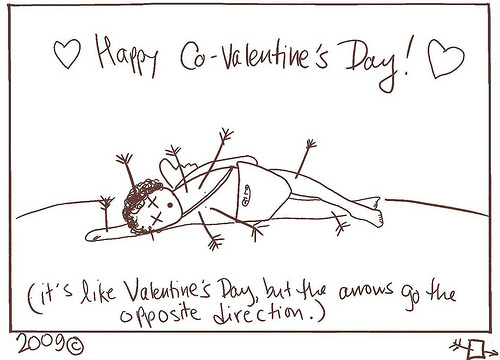
\includegraphics[height=3.3cm]{images/happy-co-valentine}}

\includegraphics[height=3.3cm]{images/homer-the-end}
\href{http://brownsharpie.courtneygibbons.org/?p=1253}{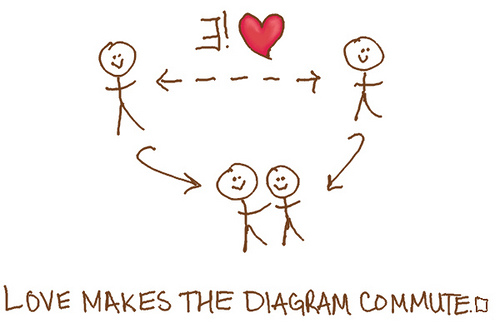
\includegraphics[height=3.3cm]{images/love-commute}}
\par

\end{document}
